\section{Description générale} %2

{\client}, une entreprise spécialisée dans les tests de systèmes embarqués véhicule, souhaite développer un démonstrateur CAN \textit{simulator in the loop} pour permettre à ses équipes de monter en compétences sur le réseau CAN. 

\vspace{\baselineskip} % saut d'une ligne
L'objectif est également de fournir une visualisation concrète de l'architecture du véhicule, du réseau CAN et du démonstrateur CAN pour les personnes novices dans le métier, tels que les nouveaux salariés lors de leur arrivé chez {\client}, ou des étudiants lors des forums. 

\vspace{\baselineskip} % saut d'une ligne
Pour répondre à ce besoin, {\client} souhaite pouvoir utiliser un Simulateur de tableau de bord sur Linux (type ICSim) et/ou un Banc de test physique, connecté(s) à une carte électronique de type Raspberry Pi pour permettre la connexion au réseau CAN. 

\vspace{\baselineskip} % saut d'une ligne
De plus, {\client} souhaite contrôler le système à distance via une application Android sur Smartphone appelée {\nomApplication}. Le Smartphone sera connecté au système (via la Raspberry Pi) par un réseau TCP/IP. Sur l'application, il sera possible d'ajouter et  d'envoyer des trames mais également d'observer toutes les trames diffusées sur le bus CAN. Il sera possible d'enregistrer les trames diffusées sur le bus CAN dans un fichier de logs présent sur la Raspberry Pi.

\vspace{\baselineskip} % saut d'une ligne
En outre, l'entreprise souhaite pouvoir injecter des fautes dans Tableau de Bord afin d'en assurer le bon fonctionnement. Elle pourra réaliser cela en envoyant des trames qui seront susceptibles de mettre Tableau de Bord en erreur, et ainsi, en vérifier le comportement.

\subsection{Caractéristiques des acteurs}
Par le terme d’acteur, nous désignons tout rôle joué par une entité (morale ou physique) qui interagit directement ou non avec le SàE. Cette entité peut être une personne (généralement un utilisateur du système) ou un autre système. 

\vspace{\baselineskip} % saut d'une ligne
Nous distinguons les acteurs dits directs (qui interagissent directement avec le SàE) et les acteurs dits indirects (qui n’ont pas d’interaction directe avec le SàE) mais qui sont à l’origine d’exigences à respecter par le SàE.

\subsubsection{Acteurs directs}
Les acteurs directs : 
\vspace{0.2cm} % ajout d'un espace vertical
\begin{itemize} 
    \item \textbf{Utilisateur} : utilisateur principal du SàE. Celui-ci a la possibilité d'envoyer et de recevoir des trames CAN grâce à l'application {\nomApplication}.
\end{itemize}
\subsubsection{Acteurs indirects}
\vspace{0.2cm} % ajout d'un espace vertical
\begin{itemize} 
    \item \textbf{N.A}
\end{itemize}

\subsection{Environnement}

% ----------------------------------------------
% ARCHITECTURE MATERIELLE ET LOGICIELLE {p.TODO}
% ----------------------------------------------
\subsubsection{Architecture matérielle et logicielle}
Le diagramme de déploiement UML de la figure \ref{schema_arch_mat} du projet représente l'architecture matérielle et logicielle du SàE. Les conventions graphiques utilisées sont explicitées sur la figure \ref{schema_legende_diag_deploiment}. Ce diagramme de déploiement identifie les entités matérielles et/ou logicielles avec lesquelles le SàE doit intéragir et permet ainsi de déterminer les principaux échanges qu'il entretient avec son environnement. 
\begin{figure}[ht] 
    \centering
    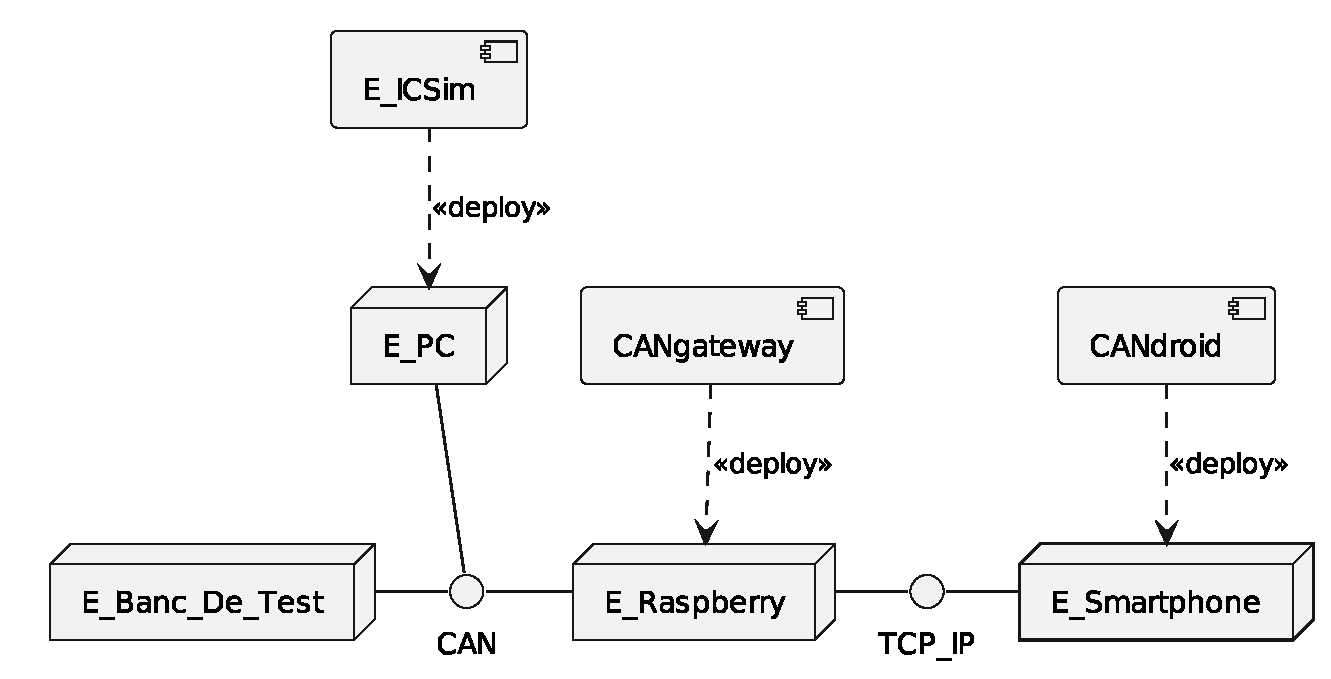
\includegraphics[width=14cm]{../schemas/arch_mat}
    \captionsetup{justification=centering}
    \caption{Architecture matérielle et logicielle représentée \\par un diagramme de déploiement UML}
    \label{schema_arch_mat}
\end{figure}

Comme indiqué sur le diagramme, l'application {\nomApplication} est déployée sur E\_Smartphone. Le programme {\nomLogiciel} est déployé sur E\_Raspberry. E\_Smartphone et E\_Raspberry communiquent ensemble grâce au protocole \hyperref[tcp_ip]{TCP/IP}. E\_Raspberry récupère les trames CAN émisent par E\_PC et/ou E\_Banc\_De\_Test grâce au RS485 CAN Hat qui permet à E\_Raspberry d'utiliser le protocole de communication CAN (Voir section \ref{dictionnaire}). E\_ICSim est un logiciel de simulation déployé sur E\_PC. Il permettra aux futurs utilisateurs de se former aux protocoles de communication CAN sans avoir à utiliser un Banc de test encombrant. Par convention, le nom de ces entités est préfixé par les caractères {\guillemotleft} E\_ {\guillemotright} (E pour Extern). Les caractéristiques de ces entités sont décrites dans le dictionnaire du domaine (voir section \ref{dictionnaire}).
\begin{figure}[ht] 
    \centering
    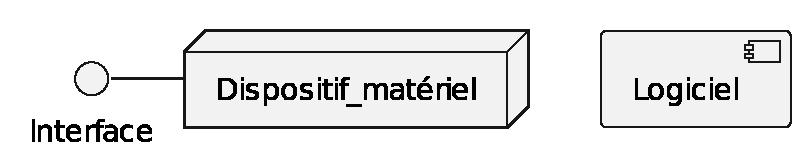
\includegraphics[width=10cm]{../schemas/legende_diag_deploiement}
    \caption{Légende du diagramme de déploiement UML}
    \label{schema_legende_diag_deploiment}
\end{figure}

\bigskip

% TODO relire et modifier les warnings
\newpage
\subsubsection{Les interfaces du système}
Cette section décrit les entrées et sorties dites « logiques » et « physiques » du SàE.
En effet, nous différencions dans cette étude deux grands types d'entrées/sorties : 
\begin{itemize}
  \item Celles dites de haut niveau (dites aussi logiques) qui décrivent les données échangées et événements entre Utilisateur, le SàE et E\_TableauDeBord. Les entrées/sorties logiques seront décrites à la section \ref{interfaces_logiques}.
  \item Celles dites de bas niveau (dites aussi physiques) qui sont les entrées/sorties réellement échangées entre le SàE et E\_TableauDeBord. Les entrées/sorties physiques 
  (ou bas niveau) seront décrites au chapitre \ref{interfaces_physiques}.
\end{itemize}

\paragraph{Les interfaces logiques}
\label{interfaces_logiques}
Le SàE est constitué d'une application Android nommée {\nomApplication} et un programme embarqué sur la Raspberry Pi nommé {\nomLogiciel}. 

\vspace{6pt}

La figure \ref{schema_contexte_log} présente le contexte en faisant figurer les entrées/sorties logiques. Cette représentation du contexte est sous la forme d'un diagramme de communication UML. Les éléments soulignés correspondent à des ensembles de messages qui vont être détaillés. \\

\begin{figure}[ht] 
    \centering
    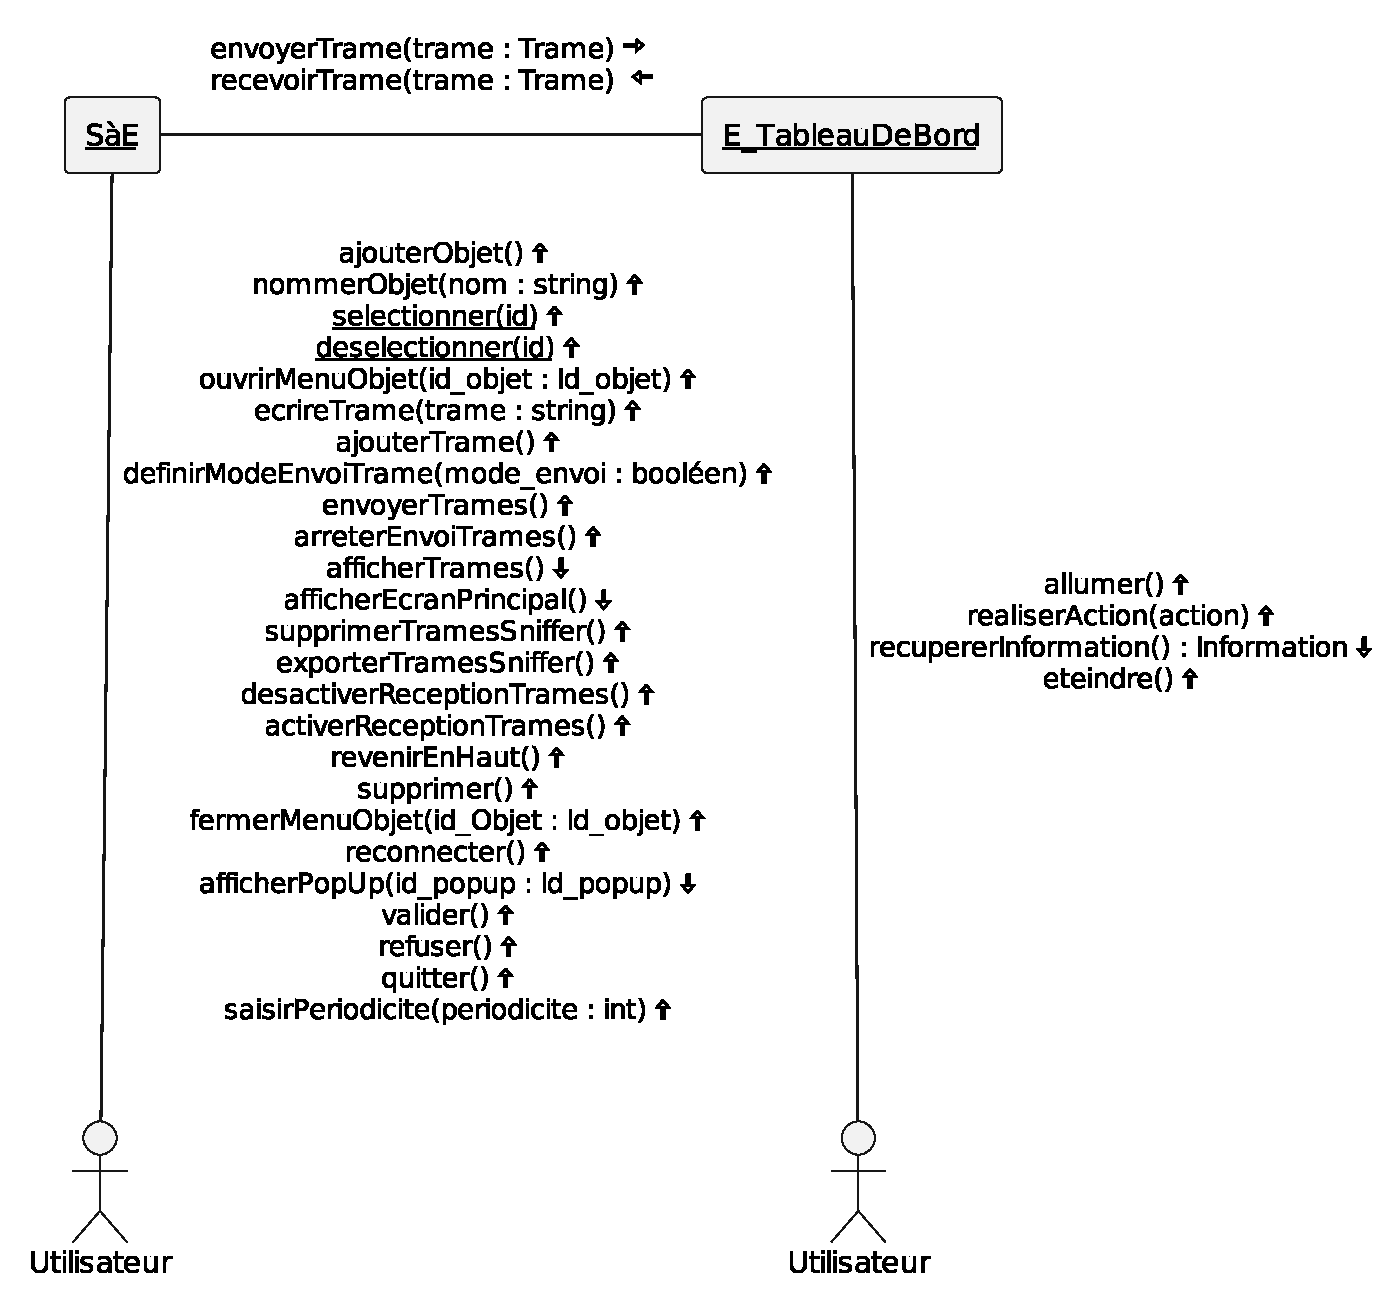
\includegraphics[width=12cm]{../schemas/contexte_log}
    \caption{Contexte logique représenté par un\\diagramme de communication UML}
    \label{schema_contexte_log}
\end{figure}

\newpage

\paragraph{Les interfaces avec les acteurs} 
L'acteur Utilisateur est en contact direct avec le SàE et Tableau de Bord. Les entrées et sorties entre Utilisateur et le SàE font référence aux fonctionnalités présentes sur l'IHM. Ces fonctionnalités sont décrites en détails dans la partie Exigences spécifiques (cf. section \ref{exigences_specifiques}). \\

Les listes d'objets et de trames mentionnées dans les descriptions suivantes sont initialement vides lors du premier lancement de l'application, mais elles sont affichées sur l'IHM. Nous allons maintenant détailler ces entrées et sorties logiques.

\vspace{-1cm}
\subparagraph{En provenance de Utilisateur}
\vspace{1cm}
\mbox{}\\

\textbf{Vers le SàE :} \vspace{0.2cm}\\ %SUBSUBPARAGRAPHE ?
\textbf{ajouterObjet()} --- Utilisateur ajoute un nouvel objet, un pop-up s'affiche ensuite pour nommer l'objet et valider l'ajout. \\
\textbf{nommerObjet(nom : string) } --- Utilisateur nomme l'objet créé dans le pop-up qui s'est affiché. Une validation est attendue. \\
\textbf{ \underline{selectionner(id)}} : 
\begin{itemize}
    \item \textbf{selectionnerObjet(id\_objet : Id\_objet)} --- Utilisateur sélectionne un objet d'ID id\_objet, il se grise ensuite. 
    \item \textbf{selectionnerTrame(id\_trame : Id\_trame)} --- Utilisateur sélectionne une trame d'ID id\_trame, elle se grise ensuite. 
\end{itemize}
\textbf{ \underline{deselectionner(id)}} : 
\begin{itemize}
    \item \textbf{deselectionnerObjet(id\_objet : Id\_objet)} --- Utilisateur désélectionne un objet d'ID id\_objet, il se dégrise ensuite. 
    \item \textbf{deselectionnerTrame(id\_trame : Id\_trame)} --- Utilisateur désélectionne une trame d'ID id\_trame, elle se dégrise ensuite. Lorsqu'il quitte le {\guillemotleft} Mode Envoi {\guillemotright}, les trames se désélectionnent automatiquement. 
\end{itemize}
\textbf{ouvrirMenuObjet(id\_objet : Id\_objet)} --- Utilisateur ouvre le menu déroulant d'un objet d'ID id\_objet. \\
\textbf{ecrireTrame(trame : string)} --- Utilisateur écrit une trame dans le menu déroulé d'un objet, le format de la trame est détaillé dans le dictionnaire de domaine (section \ref{dictionnaire}). \\
\textbf{ajouterTrame()} --- Utilisateur ajoute la trame écrite, un pop-up s'affiche pour définir le Mode Envoi de la trame.\\
\textbf{definirModeEnvoiTrame(mode\_envoi : booléen)} --- Utilisateur définit un Mode Envoi pour la trame à ajouter. Si vrai, l'envoi est ponctuel. Si faux, l'envoi est cyclique. Une validation est attendue. \\
\textbf{envoyerTrames()} --- Utilisateur demande à envoyer la ou les trames préalablement ajoutées(s) et sélectionnée(s). L'application {\nomApplication} passe alors en {\guillemotleft} Mode Envoi {\guillemotright}, et Utilisateur ne peut plus supprimer de trames ou ajouter d'objets. L'envoi des trames continue même si Utilisateur met en veille l'application {\nomApplication}.  \\
\textbf{arreterEnvoiTrames()} --- Utilisateur arrête l'envoi des trames. L'application {\nomApplication} quitte le {\guillemotleft} Mode Envoi {\guillemotright} et Utilisateur a de nouveau accès aux fonctionnalités de suppression d'élément et d'ajout d'objet.\\
\textbf{supprimerTramesSniffer()} --- Utilisateur supprime l'ensemble des trames affichées dans le sniffer. \\
\textbf{exporterTramesSniffer()} --- Utilisateur demande à exporter l'ensemble des trames affichées dans le sniffer dans un fichier de logs (voir section \ref{dictionnaire}). \\
\textbf{desactiverReceptionTrames()} --- Utilisateur désactive la réception de trames, le SàE ne va plus afficher les trames en provenance de Tableau de Bord sur l'IHM. \\
\textbf{activerReceptionTrames()} --- Utilisateur demande à activer la réception des trames, L'application {\nomApplication} affiche les trames en provenance de Tableau de Bord sur l'IHM. La reception des trames continue même si Utilisateur met en veille l'application {\nomApplication}. \\
\textbf{revenirEnHaut()} --- Utilisateur revient en haut du fil de trames affichées dans le sniffer. \\
\textbf{supprimer()} --- Utilisateur supprime les trames et objets sélectionnés. Si Utilisateur a sélectionné un ou plusieurs objets, les trames ajoutées dans le menu de ces objets seront aussi supprimées. \\
Un pop-up s'affiche pour confirmer ou non la suppression. \\
\textbf{fermerMenuObjet(id\_objet : Id\_objet)} --- Utilisateur ferme le menu précédemment ouvert d'un objet d'ID id\_objet. \\
\textbf{reconnecter()} --- Utilisateur demande à reconnecter l'application {\nomApplication} au programme {\nomLogiciel}, un pop-up s'affiche et une validation est demandée. \\
\textbf{valider()} --- Utilisateur choisit de valider son action lorsque qu'un pop-up s'affiche. \\
\textbf{refuser()} --- Utilisateur choisit de refuser de réaliser son action lorsque qu'un pop-up s'affiche.\\
\textbf{quitter()} --- Utilisateur quitte l'application {\nomApplication}. \\
\textbf{saisirPeriodicite(periodicite : int)} --- Utilisateur saisit la périodicité de la trame qu'il veut envoyer en mode cyclique. \\
\textbf{demarrer\_SSH()} --- Utilisateur démarre le programme {\nomApplication}. Le démarrage s'effectue en ligne de commande via une connexionn SSH à la Raspberry Pi. \\
\textbf{quitter\_SSH()} --- Utilisateur quitte le programme {\nomApplication}. L'arrêt s'effectue en ligne de commande via une connexionn SSH à la Raspberry Pi. \\


\textbf{Vers E\_TableauDeBord :} \vspace{0.2cm} \\ %SUBSUBPARAGRAPHE !
Les fonctions décrites ci-dessous s'exécutent en arrière-plan. \\
\\
\textbf{allumer()} --- Utilisateur allume Tableau de Bord. \\
\textbf{realiserAction(action)} --- Utilisateur réalise une action sur Tableau de Bord. \\
\textbf{recupererInformation() : Information} --- Utilisateur récupère des informations sur Tableau de Bord grâce aux indicateurs visuels. \\
\textbf{eteindre()} --- Utilisateur éteint Tableau de Bord.

\subparagraph{En provenance du SàE}
\mbox{}\\\\
\textbf{Vers Utilisateur :} \vspace{0.2cm} \\ %SUBSUBPARAGRAPHE !
\textbf{afficherEcranPrincipal()} --- L'application {\nomApplication} affiche l'écran principal. \\
\textbf{afficherTrames()} --- L'application {\nomApplication} affiche toutes les trames du sniffer, c'est-à-dire les trames qu'il a sniffées en provenance de Tableau de Bord, et les trames que Utilisateur a envoyées.  \\
\textbf{afficherPopUp(id\_popup : Id\_popup)} --- L'application {\nomApplication} affiche un pop-up d'ID id\_popup correspondant à l'action réalisée précédemment par Utilisateur (voir section \ref{dictionnaire}). \\

\textbf{Vers E\_TableauDeBord :} \vspace{0.2cm} \\ %SUBSUBPARAGRAPHE !
\textbf{envoyerTrame(trame : Trame)} --- Le SàE transmet à Tableau de Bord les trames que Utilisateur a décidé d'envoyer (voir section \ref{dictionnaire} pour les détails sur le type Trame).
\subparagraph{En provenance de E\_TableauDeBord}
\mbox{}\\

\textbf{Vers le SàE :} \vspace{0.2cm} \\ %SUBSUBPARAGRAPHE !
\textbf{recevoirTrame(trame : Trame)} --- Le SàE reçoit des trames envoyées par Tableau de Bord (voir section \ref{dictionnaire} pour les détails sur le type Trame).

\paragraph{Les interfaces physiques}
\label{interfaces_physiques}
Ce paragraphe précise les caractéristiques de chaque interface entre le logiciel et les composants matériels du
système. Il s'agit des entrées/sorties physiques. Ce sont celles que devra réellement traiter le SàE 
en les interprétant ou les générant en événement logiques. \\

La figure \ref{schema_contexte_phy} représente ce contexte physique avec un diagramme de communication UML.

\begin{figure}[ht] 
    \centering
    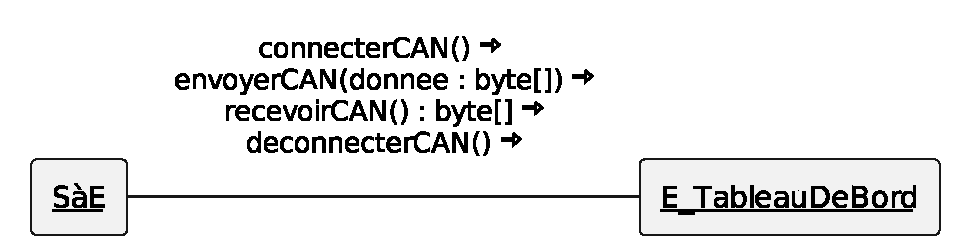
\includegraphics[width=14cm]{../schemas/contexte_phy}
    % \captionsetup{justification=centering}
    \caption{Contexte physique représenté \\par un diagramme de déploiement UML}
    \label{schema_contexte_phy}
\end{figure}

\subparagraph{En provenance du SàE}
\mbox{}\\

\textbf{Vers E\_TableauDeBord :} \vspace{0.2cm} \\ %SUBSUBPARAGRAPHE !
\textbf{connecterCAN()} --- Le SàE se connecte au bus CAN. \\
\textbf{envoyerCAN(donnee : byte[])} --- Le SàE envoie une ou plusieurs trames sur le bus CAN. \\
\textbf{recevoirCAN() : byte[] }--- Le SàE récupère la ou les trames sortantes de Tableau de Bord sur le bus CAN.  \\
\textbf{deconnecterCAN()} --- Le SàE se déconnecte du bus CAN. \\



% --------------------------
% CAS D'USAGE {p.12}
% --------------------------
%TODO
\newpage
\subsection{Fonctions principales développées}
Ce chapitre présente les principales fonctionnalités développées dans l'incrément 1 et 2 en utilisant une approche basée sur les cas d'usage et les cas d'utilisation (CU). Il met en évidence les fonctionnalités clés implémentées dans ces deux incréments, en les reliant aux cas d'usage et aux cas d'utilisation pertinents. 

\subsubsection{Rappel sur les cas d'usage}
Les cas d'usage recensent les étapes essentielles du cycle de vie d'un produit depuis la fabrication du produit jusqu'à l'élimination ou le recyclage du produit. \`A chaque étape du cycle de vie correspond un cas d'usage (si cette étape induit des fonctionnalités à définir pour le produit considéré). Pour chaque cas d'usage, plusieurs cas d'utilisation distincts peuvent être définis.\\
\newline
Parmi les cas d'usage, on retrouve généralement ceux de fabrication du produit (comprenant ou non les activités de test du produit fabriqué), de conditionnement (paramétrage éventuel, expédition et transport), de commercialisation (paramétrage éventuel, mode de démonstration, installation sur site...), d'utilisation (par le ou les utilisateurs), de maintenance (SAV ou diagnostique), de désinstallation et de recyclage (élimination ou valorisation).
\medskip

\subsubsection{Rappel sur les cas d'utilisation}
\medskip
Un cas d'utilisation (CU) représente un ensemble d'interactions entre un ou des acteurs et le système à spécifier. Ce cas d'utilisation est souvent lié à un ou parfois plusieurs cas d'usage. Un CU est principalement décrit par un scénario d'utilisation (nommé scénario nominal), scénario d'une utilisation représentative du système. Ces CU sont ensuite détaillés jusqu'à un niveau de décomposition suffisant pour décrire les fonctions attendues du système. 
\medskip

\paragraph{Représentation graphique des CU}
%~\par
Les CU peuvent être représentés sous forme graphique, voir la figure \ref{schema_diag_cu} pour un exemple. Les acteurs directs sont représentés sous forme de petits personnages. Dans les bulles, sont représentés les cas d'utilisation. Un trait entre un acteur et un CU indique que l'acteur participe à ce CU. Les liens hachurés entre CU, étiquetés par le mot <<use>> (ou <<include>>), indiquent que ce CU fait appel à l'autre CU --- on parle alors de sous-cas d'utilisation. Les liens hachurés entre CU, étiquetés par le mot <<extend>>, indique qu'il s'agit d'une extension d'un CU : un CU qui ne se déclenche que sous certaines conditions.

\begin{minipage}{1\linewidth} 
    \centering
    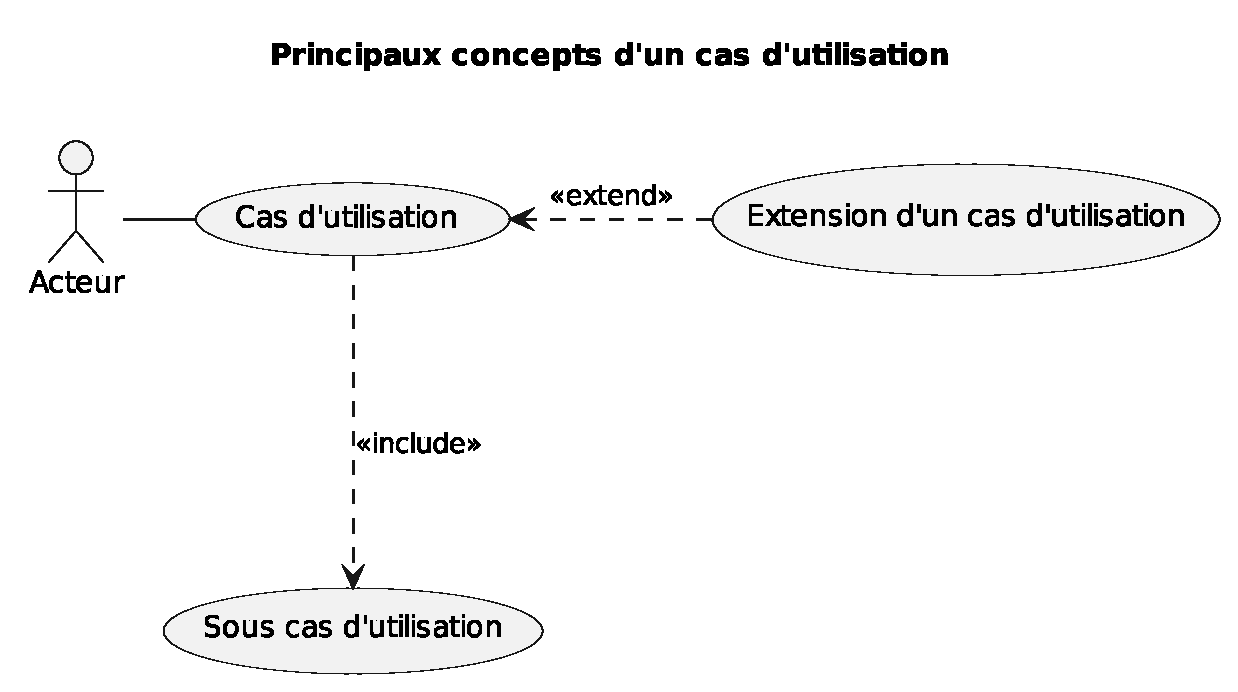
\includegraphics[width=14cm]{../schemas/exemple_diag_cu}
    \captionsetup{justification=centering}
    \captionof{figure}{Légende explicative d'un diagamme de cas d'utilisation UML}
    \label{schema_diag_cu}
\end{minipage}

\paragraph{Représentation textuelle des CU}
%~\par
La description textuelle des cas d'utilisation est souvent présentée sous forme d'un tableau constitué de champs suivants : 
\begin{longtable}[l]{|p{3cm}|p{11.7cm}|}
    \hline
        Titre & Rappelle en quelques mots l'objectif principal du cas d'utilisation.\\
    \hline
        Résumé & Décrit brièvement le comportement du cas d'utilisation.\\
    \hline
        Portée & Définit la portée de conception du CU (étendue spatiale).\\
    \hline
        Niveau & Niveau de granularité du cas d'utilisation (stratégique, utilisateur ou sous-fonction).\\
    \hline
        Acteurs directs & Acteurs qui participent au CU.\\
    \hline 
        Acteurs indirects & Acteurs qui ne participent pas au CU, mais qui ont un intérêt dans sa réalisation.\\
    \hline
        Préconditions & Ensemble des conditions qui doivent être vérifiées avant le déroulement du CU. Les
        préconditions, sans mention contraire explicite, des CU parents au CU doivent
        toujours être vérifiées.\\
    \hline
        Garanties \newline minimales & Définissent ce qui est garanti par le système à l'étude même en cas d'échec du cas d'utilisation.\\
    \hline
        Garanties en cas de succès & Définissent les garanties en cas de succès (par le scénario nominal ou par ses
        variantes). \\
    \hline
        Scénario nominal & C'est un scénario représentatif de l'utilisation du système où tout se passe bien. Il
        se termine par la réussite des objectifs. Il peut être constitué d'une condition
        déclenchant le scénario, d'un ensemble d'étapes, d'une condition de fin, et
        éventuellement d'extensions ou de variantes. Une étape peut être une interaction
        entre acteurs, une étape de validation, ou un changement interne.\\
    \hline
        Variantes & Lorsqu'il y a plusieurs façons de procéder à une même étape sans remise en cause
        du scénario nominal.\\
    \hline
        Extensions & Définissent les autres scénarios que le scénario nominal (par exemple ceux qui se
        terminent par un échec). Ils se déclenchent sur des conditions spécifiques
        détectées par le SàE.\\
    \hline
        Informations \newline complémentaires & Informations diverses nécessaires à la compréhension du CU. \\
    \hline
\end{longtable}

% ----------------------------------------------
% CU STRATEGIQUE
% ----------------------------------------------
\newpage
\subsubsection{CU Échanger des trames CAN}
\paragraph{Description graphique}
\medskip
\begin{minipage}{1\linewidth}
    \centering
    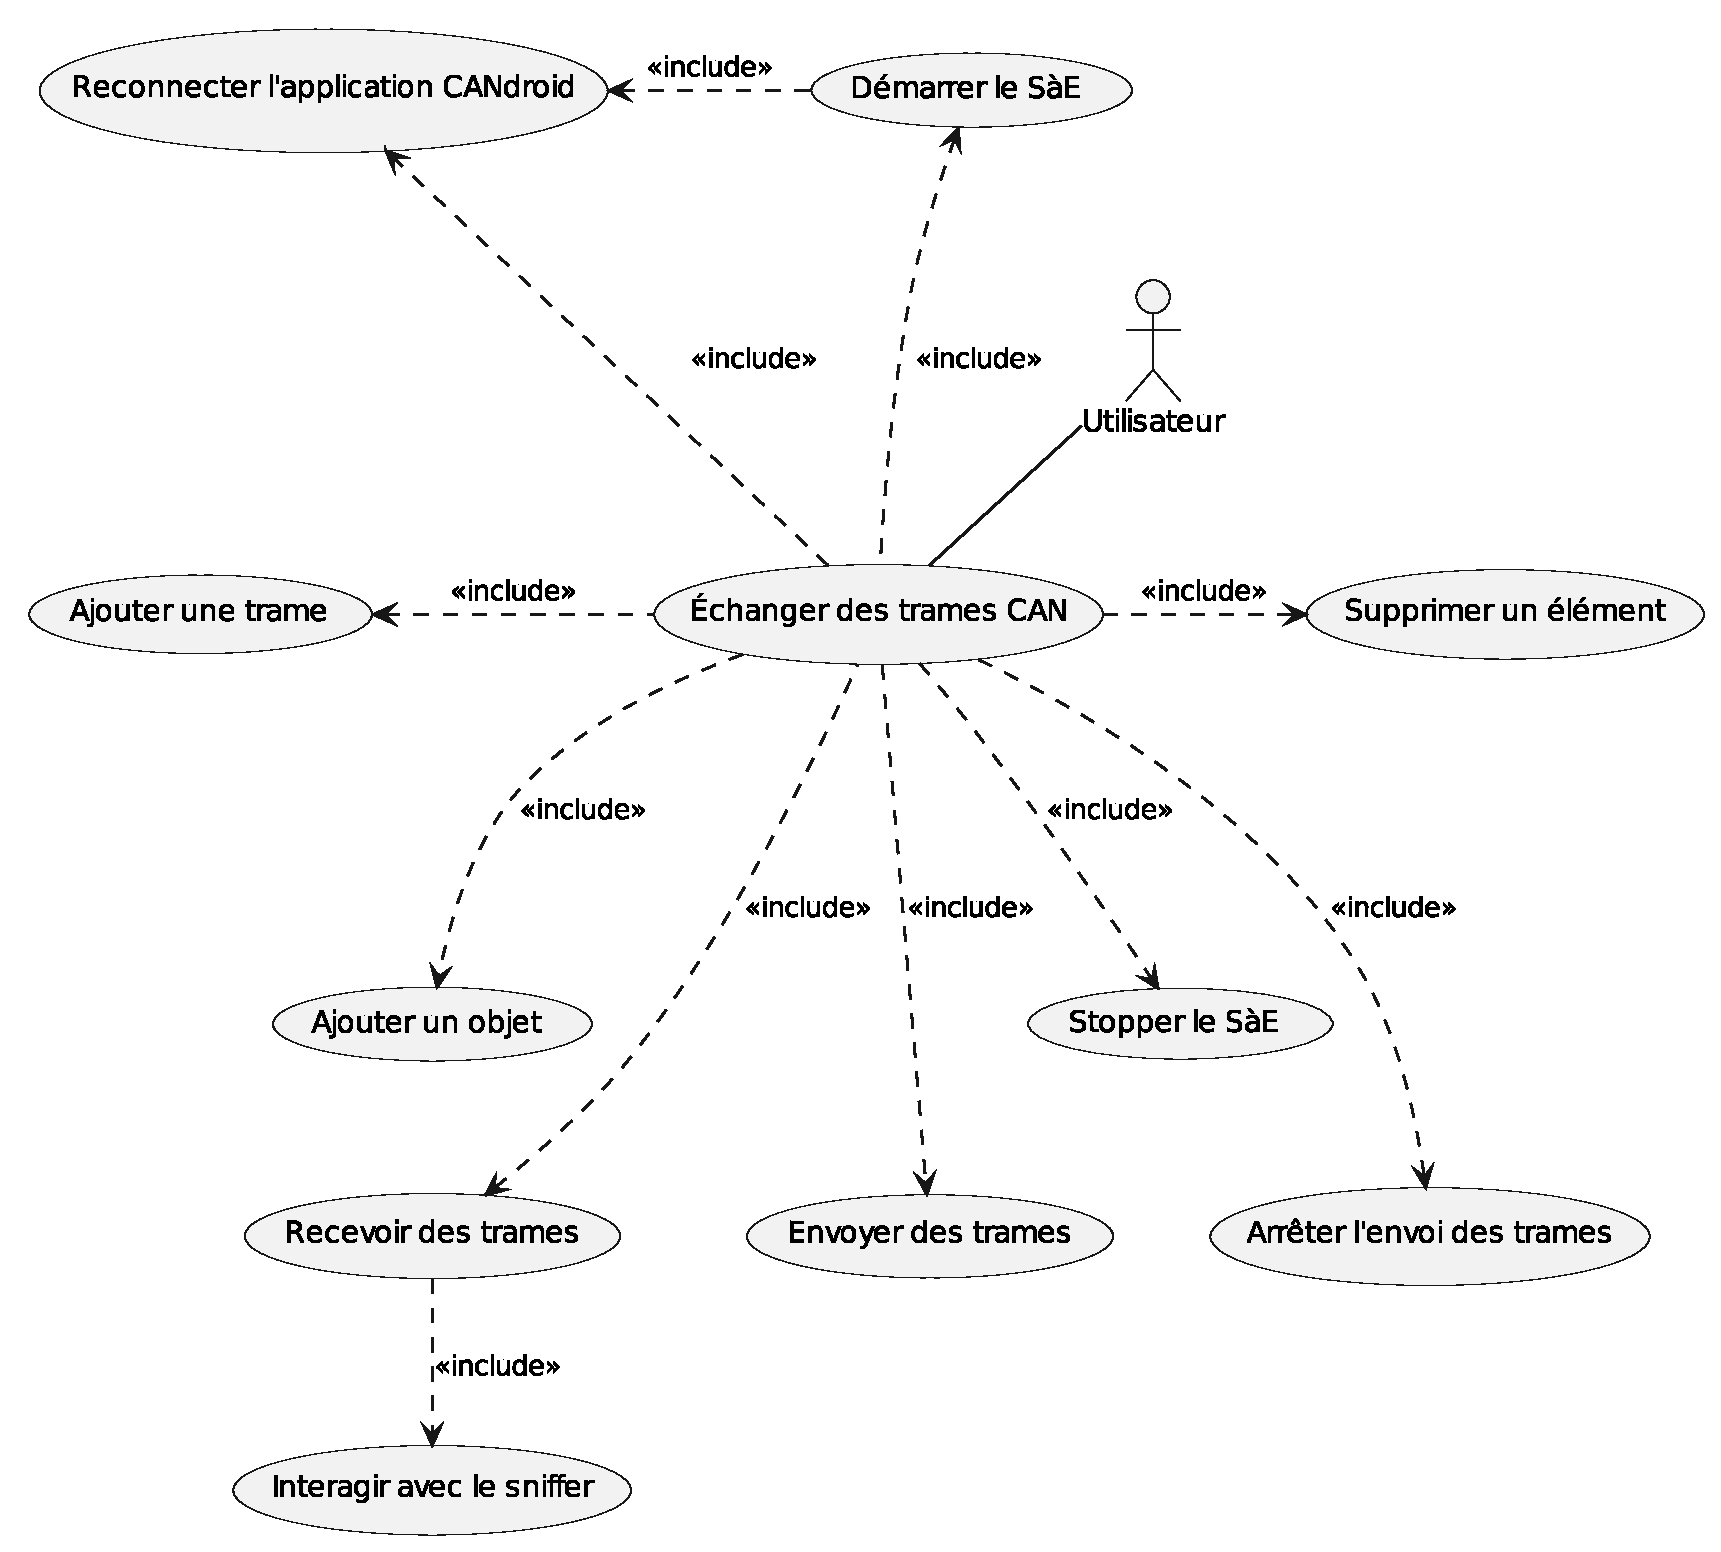
\includegraphics[width=15cm]{../../specification/schemas/cu_strat}
    \captionof{figure}{CU Échanger des trames CAN}
    \label{schema_cu_strat}
\end{minipage}

\newpage
\paragraph{Description textuelle}
\medskip

\begin{longtable}[l]{|p{3cm}|p{11.7cm}|}
    \hline
    
        Titre & Échanger des trames CAN.\\
    \hline
    
        Résumé & Utilisateur peut échanger des trames CAN avec Tableau de Bord. \\
    \hline
    
        Portée & SàE.\\
    \hline
    
        Niveau & Stratégique.\\
    \hline
    
        Acteurs directs & Utilisateur.\\
    \hline 
    
        Acteurs indirects & N.A. \\
    \hline
    
    Préconditions & 
        \begin{itemize}
            \item Tableau de Bord et la Raspberry Pi sont fonctionnels.
            \item Le programme {\nomLogiciel} est installé sur la Raspberry Pi.
            \item L'application {\nomApplication} est téléchargée sur le Smartphone.
            \item Le matériel est fonctionnel.
        \end{itemize} \\
    \hline
    
    Garanties \newline minimales & 
    \begin{itemize}
        \item L'application {\nomApplication} est utilisable.
    \end{itemize}
         \\
    \hline
    
    Garanties en cas de succès & 
    \begin{itemize}
        \item Utilisateur peut échanger des trames CAN entre Tableau de Bord et l'application {\nomApplication}.
        \item Utilisateur est capable d'observer les trames CAN reçues et d'en envoyer des nouvelles.
        \item Utilisateur est capable d'ajouter des objets ainsi que d'ajouter des trames à envoyer.
    \end{itemize}
         \\
    \hline
    
    Scénario nominal &
    \begin{enumerate}
        \item Utilisateur \underline{démarre le SàE}.
        \item Le SàE commence à \underline{recevoir des trames}.
        \item Utilisateur demande à \underline{ajouter un objet}.
        \item Utilisateur demande à \underline{ajouter une trame}.
        \item Utilisateur demande à \underline{envoyer des trames}.
        \item Le SàE diffuse les trames sur le bus CAN.
        \item Utilisateur demande à \underline{arrêter l'envoi des trames}.
        \item Utilisateur demande à \underline{supprimer un élément}.
        \item Utilisateur \underline{stoppe le SàE}.
    \end{enumerate} \\
    \hline

    Variantes & \newline
        \textbf{2,5 [La connexion n'est pas établie et Utilisateur ne souhaite pas se reconnecter]} \newline
            2,5.a.1. Va en 3. \newline
        \newline
        \textbf{2,5 [La connexion n'est pas établie \& Utilisateur souhaite se reconnecter]} \newline
            2,5.b.1. Utilisateur demande à \underline{reconnecter l'application {\nomApplication}} au programme {\nomLogiciel}. \newline
            2,5.b.2. Va en 2.\newline
        \newline
        \textbf{3,4,5,7,8 [Utilisateur souhaite stopper le SàE]}\newline
            3,4,5,7,8.a.1. Va en 9. \newline
        \newline
        \textbf{3,4,5,7,9 [Un élément existe \& Utilisateur souhaite supprimer un élément]}\newline
            3,4,5,7,9.a.1. Va en 8. \newline
        \newline
        \textbf{3,4,5,8,9 [Des trames sont en cours d'envoi \& Utilisateur souhaite arrêter l'envoi de trames]} \newline
        3,4,5,8,9.a.1. Va en 7. \newline
        \newline
        \textbf{3,4,7,8,9 [Au moins une trame existe, aucune trame n'est en cours d'envoi \& Utilisateur souhaite envoyer une trame]} \newline
        3,4,7,8,9.a.1. Va en 5. \newline
        \newline
        \textbf{3,5,7,8,9 [Utilisateur souhaite ajouter une trame \& au moins un objet existe]} \newline
        3,5,7,8,9.a.1. Va en 4. \newline
        \newline
        \textbf{4,5,7,8,9 [Utilisateur souhaite ajouter un objet]} \newline
            4,5,7,8,9.a.1. Va en 3. \newline
        \newline
        \textbf{5 [Il n'y a pas de trames à envoyer]} \newline
            5.a.1. Va en 8. \newline
        \newline
        \textbf{7 [Il n'y a pas de trames en cours d'envoi]} \newline
            7.a.1. Va en 8. \newline
        \newline
        \textbf{8 [Il n'y a pas d'éléments à supprimer]} \newline
            8.a.1. Va en 9. \newline
        \\
    \hline

    Extensions & \newline
        \textbf{2,6 [Utilisateur souhaite forcer l'arrêt du système]} \newline
        2,6.a.1. Va en 9. \newline
        \newline
        \\
    \hline
        Informations \newline complémentaires & N.A. \\
    \hline

\end{longtable}


\newpage

% ----------------------------------------------
% CU DEMARRER LE SAE
% ----------------------------------------------
\newpage
\subsubsection{CU Démarrer le SàE}
\paragraph{Description graphique}
Voir figure \ref{schema_cu_strat}.
\paragraph{Description textuelle}
\medskip

\begin{longtable}[l]{|p{3cm}|p{11.7cm}|}
    \hline
    
        Titre & Démarrer le SàE.\\
    \hline

        Résumé & Utilisateur démarre le SàE et les différents périphériques dont il a besoin. \\
    \hline

        Portée & SàE.\\
    \hline

        Niveau & Utilisateur.\\
    \hline

        Acteurs directs & Utilisateur.\\
    \hline 

        Acteurs indirects & N.A. \\
    \hline

        Préconditions & 
        \begin{itemize}
            \item Utilisateur à accès aux différents éléments du SàE ainsi que des différents périphériques dont il a besoin.
            \item Utilisateur est connecté à la Raspberry Pi en SSH.
        \end{itemize} \\ 
    \hline

        Garanties \newline minimales & N.A. \\
    \hline

        Garanties en cas de succès & 
        \begin{itemize}
            \item Utilisateur peut utiliser l'application {\nomApplication} librement. 
        \end{itemize}
        \\
    \hline
        Scénario nominal &
        \begin{enumerate}
            \item Utilisateur met en fonctionnement le Simulateur ICSim. 
            \item Utilisateur connecte la Raspberry Pi au bus CAN.
            \item Utilisateur met sous tension la Raspberry Pi.
            \item Utilisateur lance le programme {\nomLogiciel} via la \newline connexion SSH.
            \item E\_PC informe Utilisateur que le programme \newline {\nomLogiciel} est lancé.
            \item Utilisateur connecte E\_Smartphone au réseau TCP/IP de E\_Raspberry.
            \item E\_Smartphone informe Utilisateur qu'il est connecté au réseau TCP/IP de E\_Raspberry.
            \item Utilisateur démarre l'application {\nomApplication}.
            \item L'application {\nomApplication} affiche EcranPrincipal.
            \item L'application {\nomApplication} se connecte au programme \newline {\nomLogiciel}.
            \item L'application {\nomApplication} met à jour EcranPrincipal.
        \end{enumerate} \\
    \hline

    Variantes &     \newline
        \textbf{1 [Mise en fonctionnement du Banc de test uniquement]} \newline
        1.a.1. Utilisateur allume le Banc de test. \newline
        1.a.2. Va en 2. \newline
        \newline
        \textbf{1 [Mise en fonctionnement du Simulateur ICSim et du Banc de test]} \newline
        1.b.1. Utilisateur allume le Simulateur ICSim. \newline
        1.b.2. Utilisateur allume le Banc de test. \newline
        1.b.3. Va en 2. \newline
        \newline
        \textbf{1 [Utilisateur ne souhaite pas utiliser Tableau de Bord]} \newline
        1.c.1. Va en 2. \newline
        \newline
        \textbf{1-3 [Utilisateur ne souhaite pas utiliser la Raspberry Pi]} \newline
        1-3.a.1. Va en 8. \newline
        \newline
        \textbf{5 [Le programme {\nomLogiciel} ne s'est pas lancé]}\newline
        5.a.1 Utilisateur démarre l’application {\nomApplication}.\newline
        5.a.2 L’application {\nomApplication} affiche EcranPrincipal.\newline
        5.a.3 Fin du CU. \newline
        \newline
        \textbf{7 [La connexion échoue \& Utilisateur ne souhaite pas se reconnecter]} \newline
        7.a.1. Va en 8. \newline
        \newline
        \textbf{7 [La connexion échoue \& Utilisateur souhaite se reconnecter]}\newline
        7.b.1 Va en 6. \newline
        \newline
        \textbf{10 [La connexion échoue \& Utilisateur ne souhaite pas se reconnecter]} \newline
        10.a.1. Fin du CU. \newline
        \newline
        \textbf{10 [La connexion échoue \& Utilisateur souhaite se reconnecter]} \newline
        10.b.1. Utilisateur demande à \underline{reconnecter l'application {\nomApplication}} au programme {\nomLogiciel}. \newline
        10.b.2. Fin du CU. \newline
        \\
    \hline
    Extensions & N.A. \\
    \hline
    Informations \newline complémentaires & N.A. \\
    \hline
\end{longtable}

% ----------------------------------------------
% CU DEMARRER LE SAE
% ----------------------------------------------
\newpage
\subsubsection{CU Reconnecter l'application {\nomApplication}}
\paragraph{Description graphique}
\medskip
Voir figure \ref{schema_cu_strat}.
\paragraph{Description textuelle}
\medskip

\begin{longtable}[l]{|p{3cm}|p{11.7cm}|}
    \hline
    
        Titre & Reconnecter l'application {\nomApplication}.\\
    \hline

        Résumé & Utilisateur peut reconnecter l'application {\nomApplication} au programme {\nomLogiciel}. \\
    \hline

        Portée & Application {\nomApplication}.\\
    \hline

        Niveau & Utilisateur.\\
    \hline

        Acteurs directs & Utilisateur.\\
    \hline 

        Acteurs indirects & N.A. \\
    \hline

        Préconditions & 
        \begin{itemize}
            \item L'application {\nomApplication} est déconnectée du programme \newline {\nomLogiciel}. 
        \end{itemize}
        \\
    \hline

        Garanties \newline minimales & N.A. \\
    \hline

        Garanties en cas de succès & 
        \begin{itemize}
            \item L'application {\nomApplication} est de nouveau connectée au programme {\nomLogiciel}.
            \item Utilisateur peut utiliser l’application {\nomApplication} librement.
        \end{itemize}
         \\
    \hline
        Scénario nominal &
        \begin{enumerate}
            \item Utilisateur demande la reconnexion de l'application \newline{\nomApplication} au programme {\nomLogiciel}. 
            \item L'application {\nomApplication} affiche PopupDemandeReconnexion.
            \item Utilisateur valide la reconnexion.
            \item L'application {\nomApplication} affiche EcranPrincipal.
            \item L'application {\nomApplication} se reconnecte au programme \newline {\nomLogiciel}.
            \item L'application {\nomApplication} met à jour EcranPrincipal.
        \end{enumerate} \\
    \hline

    Variantes &     \newline
        \textbf{3 [Utilisateur souhaite abandonner la reconnexion]} \newline
        3.a.1. Utilisateur annule la reconnexion. \newline
        3.a.2. L'application {\nomApplication} affiche EcranPrincipal. \newline
        3.a.3. Fin du CU.\newline
        \newline
        \textbf{5 [La connexion échoue \& Utilisateur ne souhaite pas se reconnecter]} \newline
        5.a.1. Fin du CU. \newline
        \newline
        \textbf{5 [La connexion échoue \& Utilisateur souhaite se reconnecter]} \newline
        5.b.1. Va en 1. \newline
        \\
    \hline

        Extensions & N.A. \\
    \hline
    Informations \newline complémentaires & N.A. \\
    \hline
\end{longtable}

% ----------------------------------------------
% CU Recevoir des trames
% ----------------------------------------------
\newpage
\subsubsection{CU Recevoir des trames}
\paragraph{Description graphique}
Voir figure \ref{schema_cu_strat}.
\medskip
\paragraph{Description textuelle}
\medskip

\begin{longtable}[l]{|p{3cm}|p{11.7cm}|}
    \hline
    
        Titre & Recevoir des trames.\\
    \hline

        Résumé & L'application {\nomApplication} reçoit et affiche les trames du réseau CAN. \\
    \hline

        Portée & Application {\nomApplication}.\\
    \hline

        Niveau & Utilisateur.\\
    \hline

        Acteurs directs & Utilisateur.\\
    \hline 

        Acteurs indirects & N.A. \\
    \hline

        Préconditions & 
            \begin{itemize}
                \item Le SàE est démarré. 
                \item L'application {\nomApplication} est connectée au programme \newline {\nomLogiciel}.
                \item La Raspberry Pi est connectée au bus CAN.
                \item Tableau de Bord est connecté au bus CAN.
            \end{itemize}\\
    \hline

        Garanties \newline minimales & N.A. \\
    \hline

        Garanties en cas de succès & 
        \begin{itemize}
            \item Les trames sont affichées sur le sniffer de l'application \newline {\nomApplication}.
        \end{itemize}
        \\
    \hline

        Scénario nominal &
        \begin{enumerate}
            \item Utilisateur commande un actionneur sur Tableau de Bord.
            \item Le SàE récupère les trames du réseau CAN.
            \item L'application {\nomApplication} met à jour EcranPrincipal.
            \item Utilisateur demande à \underline{interagir avec le sniffer}.
        \end{enumerate} \\
    \hline

        Variantes & \newline
            \textbf{1-2 [La connexion échoue \& Utilisateur ne souhaite pas se reconnecter]} \newline
            1-2.a.1. Va en 3. \newline
            \newline
            \textbf{1-2 [La connexion échoue \& Utilisateur souhaite se reconnecter]} \newline
            1-2.b.1. Utilisateur demande à \underline{reconnecter l'application {\nomApplication}} au programme {\nomLogiciel}. \newline
            1-2.b.2. Va en 1. \newline
            \newline
            \textbf{4 [Utilisateur souhaite commander un autre actionneur]}\newline
            4.a.1. Va en 1. \newline
            \\
    \hline

        Extensions & \newline
        \textbf{2-3 [Utilisateur a demandé l'arrêt de la réception de trames]}
        2-3.a.1. Fin du CU. \newline
        \\
    \hline
    Informations \newline complémentaires & N.A. \\
    \hline
\end{longtable}

% ----------------------------------------------
% CU Interagir avec le sniffer
% ----------------------------------------------
\newpage
\subsubsection{CU Interagir avec le sniffer}
\paragraph{Description graphique}
Voir figure \ref{schema_cu_strat}.
\paragraph{Description textuelle}
\medskip

\begin{longtable}[l]{|p{3cm}|p{11.7cm}|}
    \hline
    
        Titre & Interagir avec le sniffer.\\
    \hline

        Résumé & Utilisateur interagit avec le sniffer. \\
    \hline

        Portée & Application {\nomApplication}.\\
    \hline

        Niveau & Utilisateur.\\
    \hline

        Acteurs directs & Utilisateur.\\
    \hline 

        Acteurs indirects & N.A. \\
    \hline

        Préconditions & 
            \begin{itemize}
                \item Le SàE est démarré. 
                \item L'application {\nomApplication} est connectée au programme \newline {\nomLogiciel}.
                \item La Raspberry Pi est connectée au bus CAN.
                \item Tableau de Bord est connecté au bus CAN.
            \end{itemize}\\
    \hline

        Garanties \newline minimales & N.A. \\
    \hline

        Garanties en cas de succès & 
        \begin{itemize}
            \item Utilisateur est capable d'exporter et de supprimer les trames du sniffer.
            \item Utilisateur est capable d'arrêter la mise à jour du sniffer en temps réel et de revenir en haut du fil lorsqu'il fait défiler les trames.
        \end{itemize}
        \\
    \hline

        Scénario nominal & 
        \begin{enumerate}
            \item Utilisateur demande de revenir en haut du fil.
            \item L'application {\nomApplication} va en haut du fil.
            \item Utilisateur demande d'effacer les trames.
            \item L'application {\nomApplication} efface les trames affichées.
            \item Utilisateur demande l'arrêt de la réception des trames.
            \item L'application {\nomApplication} stoppe l'affichage de nouvelles trames.
            \item Utilisateur demande d'enregistrer les trames reçues sur le \newline Smartphone.
            \item L'application {\nomApplication} enregistre les trames dans un fichier de log (voir section \ref{dictionnaire}).
            \item Utilisateur demande la reprise de la réception des trames.
            \item L'application {\nomApplication} reprend l'affichage de nouvelles trames.
        \end{enumerate} \\
    \hline

        Variantes & \newline
            \textbf{1,3,5,7 [La réception de trames est arrêtée \& Utilisateur souhaite reprendre la réception de trames]}\newline
                1,3,5,7.a.1. Va en 9. \newline
            \newline
            \textbf{1,3,5,7,9 [Utilisateur ne souhaite rien faire]}\newline
                1,3,5,7,9.a.1. Fin du CU. \newline
            \newline
            \textbf{1,3,9 [La réception de trames est arrêtée \& Utilisateur souhaite enregistrer les trames reçues]}\newline
                1,3,9.a.1. Va en 7. \newline
            \newline
            \textbf{1,3,9 [La réception de trames est en cours \& Utilisateur souhaite arrêter la réception de trames]}\newline
                1,3,9.b.1. Va en 5. \newline
            \newline
            \textbf{1,3,9 [La réception de trames est en cours \& Utilisateur souhaite enregistrer les trames reçues]}\newline
                1,3,9.c.1. Va en 5. \newline
            \newline
            \textbf{1,5,7,9 [Utilisateur souhaite effacer les trames]}\newline
                1,5,7,9.a.1. Va en 3. \newline
            \newline
            \textbf{3,5,7,9 [Utilisateur souhaite aller en haut du fil]}\newline
                3,5,7,9.a.1. Va en 1. \newline
            \\
    \hline

        Extensions & N.A. \\
    \hline
    Informations \newline complémentaires & N.A. \\
    \hline
\end{longtable}

% ----------------------------------------------
% CU CREER UN NOUVEL OBJET
% ----------------------------------------------
\newpage
\subsubsection{CU Ajouter un objet}
\paragraph{Description graphique}
Voir figure \ref{schema_cu_strat}.
\paragraph{Description textuelle}
\medskip

\begin{longtable}[l]{|p{3cm}|p{11.7cm}|}
    \hline
    
        Titre & Ajouter un objet.\\
    \hline

        Résumé & Utillisateur ajoute un objet sur l'application {\nomApplication}. \\
    \hline

        Portée & Application {\nomApplication}.\\
    \hline

        Niveau & Utilisateur. \\
    \hline

        Acteurs directs & Utilisateur.\\
    \hline 

        Acteurs indirects & N.A. \\
    \hline

        Préconditions & 
        \begin{itemize}
            \item L'application {\nomApplication} est démarrée.
        \end{itemize} \\
    \hline

        Garanties \newline minimales & N.A. \\
    \hline

        Garanties en cas de succès & 
        \begin{itemize}
            \item Un objet est ajouté. 
        \end{itemize}
        \\
    \hline

    Scénario nominal &
    \begin{enumerate} 
        \item Utilisateur demande l'ajout d'un objet. 
        \item Le SàE choisit un Nom d'objet par défaut.
        \item L'application {\nomApplication} affiche PopupAjoutObjet.
        \item Utilisateur saisit un nom d'objet.
        \item Utilisateur valide l'ajout.
        \item L'application {\nomApplication} met à jour EcranPrincipal.
    \end{enumerate} \\
    \hline

        Variantes & \newline
        \textbf{2 [Nombre maximal d'objets atteint \& Utilisateur souhaite ajouter un objet]} \newline
        2.a.1. L’application {\nomApplication} affiche PopupErreurNombreObjet. \newline 
        2.a.2. Utilisateur ferme PopupErreurNombreObjet. \newline
        2.a.3. L’application {\nomApplication} affiche EcranPrincipal. \newline
        2.a.4. Fin du CU. \newline
        \newline
        \textbf{4 [Utilisateur ne souhaite pas saisir de nom]} \newline
        4.a.1. Va en 5. \newline
        \newline
        \textbf{6 [Utilisateur souhaite saisir un nom qui existe déjà]} \newline
        6.a.1. L'application {\nomApplication} affiche PopupErreurAjoutObjet. \newline
        6.a.2. Va en 4. \newline
        \\
    \hline

        Extensions & \newline
        \textbf{4-5 [Utilisateur souhaite annuler]} \newline
        4-5.a.1. Utilisateur ferme PopupAjoutObjet. \newline
        4-5.a.2. L’application {\nomApplication} affiche EcranPrincipal. \newline
        4-5.a.3. Fin du CU. \newline
        \\
    \hline
    Informations \newline complémentaires & N.A. \\
    \hline
\end{longtable}

% ----------------------------------------------
% CU Enregistrer des trames CAN
% ----------------------------------------------
\newpage
\subsubsection{CU Ajouter une trame}
\paragraph{Description graphique}
Voir figure \ref{schema_cu_strat}.
\paragraph{Description textuelle}
\medskip

\begin{longtable}[l]{|p{3cm}|p{11.7cm}|}
    \hline
    
        Titre & Ajouter une trame.\\
    \hline

        Résumé & Utilisateur ajoute une trame CAN associée à un objet avec son Mode Envoi. \\
    \hline

        Portée & Application {\nomApplication}.\\
    \hline

        Niveau & Utilisateur.\\
    \hline

        Acteurs directs & Utilisateur.\\
    \hline 

        Acteurs indirects & N.A. \\
    \hline

        Préconditions & 
        \begin{itemize}
            \item Le SàE est démarré.
            \item Un objet existe.
        \end{itemize} \\
    \hline

        Garanties \newline minimales & N.A.\\
    \hline

        Garanties en cas de succès & 
        \begin{itemize}
            \item Une trame est créée dans le bon objet.
        \end{itemize}
         \\
    \hline

        Scénario nominal &
        \begin{enumerate}
            \item Utilisateur déroule le menu de l'objet.
            \item L'application {\nomApplication} met à jour EcranPrincipal.
            \item Utilisateur saisit la trame. 
            \item Utilisateur valide la saisie de la trame.
            \item L'application {\nomApplication} affiche PopupModeEnvoiTrame.
            \item Utilisateur choisit le mode d'envoi ponctuel.
            \item Utilisateur valide le mode d'envoi.
            \item L'application {\nomApplication} affiche EcranPrincipal.
        \end{enumerate} \\
    \hline

        Variantes & \newline
        \textbf{1 [L’objet est déjà déplié]} \newline
            1.a.1. Va en 3.\newline
            \newline
        \textbf{5 [Nombre maximal de trames atteint \& Utilisateur souhaite
        ajouter une trame]} \newline
            5.a.1. L’application {\nomApplication} affiche PopupErreurNombreTrame.\newline
            5.a.2. Utilisateur ferme PopupErreurNombreTrame. \newline
            5.a.3. L’application {\nomApplication} affiche EcranPrincipal. \newline
            5.a.4. Fin du CU. \newline
            \newline
        \textbf{5 [Utilisateur souhaite ajouter une trame qui n'a pas le bon format]} \newline
            5.b.1. L'application {\nomApplication} affiche PopupErreurSaisieTrame. \newline
            5.b.2. Utilisateur ferme PopupErreurSaisieTrame. \newline
            5.b.3. L’application {\nomApplication} affiche EcranPrincipal. \newline
            5.b.4. Va en 3. \newline 
            \newline 
        \textbf{6 [Utilisateur choisit le mode cyclique \& souhaite changer la périodicité]} \newline
            6.a.1. Utilisateur choisit le mode d'envoi cyclique. \newline
            6.a.2. Utilisateur saisit la périodicité. \newline
            6.a.3. Va en 7. \newline
            \newline
        \textbf{6 [Utilisateur choisit le mode cyclique \& souhaite garder la périodicité par défaut]} \newline
            6.b.1. Utilisateur choisit le mode d'envoi cyclique. \newline    
            6.b.2. Va en 7. \newline
            \\
    \hline

        Extensions & \newline
        \textbf{6-7 [Utilisateur souhaite annuler]} \newline
        6-7.a.1. Utilisateur ferme PopupModeEnvoiTrame. \newline
        6-7.a.2. L'application {\nomApplication} affiche EcranPrincipal. \newline
        \\
    \hline
    Informations \newline complémentaires & N.A. \\
    \hline
\end{longtable}

% ----------------------------------------------
% CU ENVOYER DES TRAMES
% ----------------------------------------------
\newpage
\subsubsection{CU Envoyer des trames}
\paragraph{Description graphique}
Voir figure \ref{schema_cu_strat}.

\paragraph{Description textuelle}
\medskip

\begin{longtable}[l]{|p{3cm}|p{11.7cm}|}
    \hline
    
        Titre & Envoyer des trames.\\
    \hline
    
        Résumé & Utilisateur utilise l'application {\nomApplication} afin d'envoyer une trame CAN au Tableau de Bord. \\
    \hline
    
        Portée & SàE.\\
    \hline
    
        Niveau & Utilisateur\\
    \hline
    
        Acteurs directs & Utilisateur.\\
    \hline 
    
        Acteurs indirects & N.A. \\
    \hline
    
        Préconditions & 
        \begin{itemize}
            \item Le SàE est démarré.
            \item Un ou plusieurs objets existent.
            \item Une ou plusieurs trames existent.
            \item L'application {\nomApplication} est connectée au programme \newline {\nomLogiciel}.
            \item La Raspberry Pi est connectée au bus CAN.
            \item Tableau de Bord est connecté au bus CAN.
        \end{itemize}
        \\
    \hline
    
        Garanties \newline minimales & N.A. \\
    \hline
    
        Garanties en cas de succès & 
        \begin{itemize}
            \item La trame CAN est envoyée à Tableau de Bord.
        \end{itemize}
         \\
    \hline
    
        Scénario nominal & 
        \begin{enumerate}
            \item Utilisateur déroule le menu d'un objet.
            \item L'application {\nomApplication} met à jour EcranPrincipal.
            \item Utilisateur sélectionne une trame.
            \item L'application {\nomApplication} met à jour EcranPrincipal.
            \item Utilisateur demande à envoyer la trame.
            \item Le SàE diffuse la trame sur le bus CAN.
            \item L'application {\nomApplication} met à jour EcranPrincipal.
        \end{enumerate}
        \\
    \hline
        Variantes &     \newline
        \textbf{1 [L'objet est déjà déplié]} \newline
            1.a.1. Va en 3. \newline
            \newline
        \textbf{3 [Une trame est sélectionnée \& Utilisateur ne souhaite pas sélectionner de trames]} \newline
            3.a.1. Va en 5. \newline
            \newline
        \textbf{3 [Aucune trame n'est sélectionnée \& Utilisateur ne souhaite pas sélectionner de trames]} \newline
            3.b.1. Fin du CU. \newline
            \newline
        \textbf{5 [Utilisateur souhaite sélectionner plusieurs trames]} \newline
            5.a.1. Va en 1. \newline
            \newline
        \textbf{5 [Utilisateur ne souhaite plus envoyer de trames]} \newline
            5.b.1. Utilisateur désélectionne les trames grisées. \newline
            5.b.2. L'application {\nomApplication} met à jour EcranPrincipal. \newline
            5.b.3. Fin du CU. \newline
            \newline
        \textbf{5 [Utilisateur souhaite désélectionner une trame]}\newline
            5.c.1. Utilisateur désélectionne une trame grisée. \newline
            5.c.2. L'application {\nomApplication} met à jour EcranPrincipal. \newline
            5.c.3. Va en 3. \newline
            \newline
        \textbf{6 [Une ou plusieurs trames sélectionnées sont paramétrées avec le Mode Envoi cyclique]} \newline
            6.a.1. Le SàE commence l'envoi des trames sélectionnées sur le bus CAN. \newline
            6.a.2. Va en 7. \newline
        \\
    \hline
        Extensions &  N.A. \\
     
    \hline
    Informations \newline complémentaires & N.A. \\
    \hline
\end{longtable}

% ----------------------------------------------
% CU Arreter l'envoi des trames 
% ----------------------------------------------
\newpage
\subsubsection{CU Arrêter l'envoi des trames}
\paragraph{Description graphique}
Voir figure \ref{schema_cu_strat}.

\paragraph{Description textuelle}
\medskip

\begin{longtable}[l]{|p{3cm}|p{11.7cm}|}
    \hline
    
        Titre & Arrêter l'envoi des trames.\\
    \hline
    
        Résumé & Utilisateur utilise l'application {\nomApplication} afin d'arrêter l'envoi des trames à Tableau de Bord. \\
    \hline
    
        Portée & SàE.\\
    \hline
    
        Niveau & Utilisateur.\\
    \hline
    
        Acteurs directs & Utilisateur.\\
    \hline 
    
        Acteurs indirects & N.A. \\
    \hline
    
        Préconditions & 
        \begin{itemize}
            \item Le SàE est démarré.
            \item L'application {\nomApplication} est connectée au programme \newline {\nomLogiciel}.
            \item La Raspberry Pi est connectée au bus CAN.
            \item Tableau de Bord est connecté au bus CAN.
            \item Un ou plusieurs objets existent.
            \item Une ou plusieurs trames existent.
            \item Une ou plusieurs trames sont en cours d'envoi.
        \end{itemize}
        \\
    \hline
    
        Garanties \newline minimales & N.A. \\
    \hline
    
        Garanties en cas de succès & 
        \begin{itemize}
            \item Plus aucune trame CAN n'est envoyée à Tableau de Bord.
        \end{itemize}
         \\
    \hline
    
        Scénario nominal &
        \begin{enumerate}
            \item Utilisateur demande à stopper l'envoi des trames.
            \item L'application {\nomApplication} affiche PopupArretEnvoi.
            \item Utilisateur confirme l'arrêt de l'envoi des trames.
            \item Le SàE arrête de diffuser les trames sur le bus CAN.
            \item L'application {\nomApplication} affiche EcranPrincipal.
        \end{enumerate}
        \\
    \hline
        Variantes & \newline
        \textbf{3 [Utilisateur ne souhaite plus arrêter l'envoi des trames]} \newline
            3.a.1. Utilisateur ferme le pop-up. \newline
            3.a.2. Va en 5. \newline
        \\
    \hline
        Extensions &  N.A. \\
     
    \hline
    Informations \newline complémentaires & N.A. \\
    \hline
\end{longtable}

% ----------------------------------------------
% CU Supprimer un élement 
% ----------------------------------------------
\newpage
\subsubsection{CU Supprimer un élément}
\paragraph{Description graphique}
Voir figure \ref{schema_cu_strat}.

\paragraph{Description textuelle}
\medskip

\begin{longtable}[l]{|p{3cm}|p{11.7cm}|}
    \hline
    
        Titre & Supprimer un élément.\\
    \hline
    
        Résumé & Utilisateur utilise l'application {\nomApplication} pour supprimer une trame ou un objet. \\
    \hline
    
        Portée & SàE.\\
    \hline
    
        Niveau & Utilisateur.\\
    \hline
    
        Acteurs directs & Utilisateur.\\
    \hline 
    
        Acteurs indirects & N.A. \\
    \hline
    
        Préconditions & 
        \begin{itemize}
            \item Le SàE est démarré.
            \item Un ou plusieurs objets existent.
            \item Une ou plusieurs trames existent.
            \item Aucune trame n'est en cours d'envoi.
        \end{itemize}
        \\
    \hline
    
        Garanties \newline minimales & N.A. \\
    \hline
    
        Garanties en cas de succès & 
        \begin{itemize}
            \item L'élément sélectionné est supprimé de l'application. 
        \end{itemize}
        \\
    \hline
    
        Scénario nominal &
        \begin{enumerate}
            \item Utilisateur sélectionne un objet.
            \item L'application {\nomApplication} met à jour EcranPrincipal.
            \item Utilisateur demande la suppression de la sélection.
            \item L'application {\nomApplication} affiche PopupSuppressionElement.
            \item Utilisateur valide la suppression de la sélection.
            \item L'application {\nomApplication} met à jour EcranPrincipal.
        \end{enumerate}
        \\
    \hline
        Variantes &     \newline
        \textbf{1 [Utilisateur souhaite sélectionner une trame]} \newline
            1.a.1. Utilisateur déroule le menu d'un objet. \newline
            1.a.2. Le SàE met à jour EcranPrincipal.\newline
            1.a.3. Utilisateur sélectionne une trame.\newline
            1.a.4. Va en 2.\newline
            \newline
        \textbf{3 [Utilisateur souhaite sélectionner un autre élément]} \newline
            3.a.1. Va en 1.\newline
            \newline
        \textbf{3 [Utilisateur souhaite désélectionner un élément]} \newline
            3.b.1. Utilisateur désélectionne un élément.\newline
            3.b.2. Le SàE met à jour EcranPrincipal.\newline
            3.b.3. Va en 3.\newline
            \newline
        \textbf{5 [Utilisateur ne souhaite plus supprimer d'élément]} \newline
            5.a.1. Utilisateur annule la suppression d'élément. \newline
            5.a.2. Va en 6.\newline
        \\
    \hline
        Extensions &  N.A. \\
     
    \hline
    Informations \newline complémentaires & N.A. \\
    \hline
\end{longtable}

% ----------------------------------------------
% CU STOPPER LE SAE
% ----------------------------------------------
\newpage
\subsubsection{CU Stopper le SàE}
\paragraph{Description graphique}
Voir figure \ref{schema_cu_strat}.
\paragraph{Description textuelle}
\medskip

\begin{longtable}[l]{|p{3cm}|p{11.7cm}|}
    \hline
    
        Titre & Stopper le SàE. \\
    \hline

        Résumé & Permet d'arrêter convenablement le SàE. \\
    \hline

        Portée & SàE.\\
    \hline

        Niveau & Utilisateur.\\
    \hline

        Acteurs directs & Utilisateur.\\
    \hline 

        Acteurs indirects & N.A. \\
    \hline

        Préconditions & 
        \begin{itemize}
            \item Le SàE est démarré. 
            \item Utilisateur est connecté à la Raspberry Pi en SSH.
        \end{itemize}
        \\
    \hline

        Garanties \newline minimales & N.A. \\
    \hline

        Garanties en cas de succès & 
        \begin{itemize}
            \item Le SàE est arrêté. 
        \end{itemize}
        \\
    \hline

        Scénario nominal & 
        \begin{enumerate}
            \item Utilisateur quitte l'application {\nomApplication}.
            %\item L'application {\nomApplication} se déconnecte du programme {\nomLogiciel}.
            \item Utilisateur arrête le programme {\nomLogiciel}.
            \item Utilisateur met hors tension la Raspberry Pi.
            \item Utilisateur éteint le Simulateur ICSim.
        \end{enumerate}
        \\
    \hline

    Variantes & \newline
        \textbf{2-4 [Uniquement application CANdroid en fonctionnement]} \newline
        2-4.a.1. Fin du CU. \newline
        \newline
        \textbf{4 [Utilisateur utilise le Simulateur et le Banc de test]} \newline
        4.a.1. Utilisateur éteint le Simulateur ICSim. \newline
        4.a.2. Utilisateur éteint le Banc de test. \newline
        4.a.3. Utilisateur débranche le Banc de test. \newline
        4.a.4. Fin du CU. \newline
        \newline
        \textbf{4 [Utilisateur utilise uniquement le Banc de test]} \newline
        4.b.1. Utilisateur éteint le Banc de test. \newline
        4.b.2. Utilisateur débranche le Banc de test. \newline
        4.b.3. Fin du CU. \newline
        \newline
        \textbf{4 [Aucun Tableau de Bord n'est allumé]} \newline
        4.c.1. Fin du CU. \newline
        \\
    \hline

        Extensions & N.A. \\
    \hline
    Informations \newline complémentaires & N.A. \\
    \hline
\end{longtable}




\newpage

\subsection{Contraintes}

\subsubsection{Politiques réglementaires}
Le code source ainsi que les conceptions de ce produit ne sont pas soumis à une obligation de confidentialité. Il n'y a aucune restriction ou politique réglementaire qui s'applique à ces informations. 

\subsubsection{Contraintes matérielles}
Le produit est livré fonctionnel sur un Smartphone Samsung Galaxy A20e fonctionnant sous Android 9, ainsi que sur une Raspberry Pi 3B+. La connexion est fonctionnelle avec l'utilisation du module de communication CAN PCAN.USB IPEH-002021 175459 de la marque PEAK pour E\_PC, ainsi qu'un module CAN RS485 pour E\_Raspberry.

\subsubsection{Exigences de fiabilité}
L'équipe {\teamName} s'engage à déployer les meilleurs efforts pour respecter les exigences suivantes :
\begin{itemize}
    \item Les actionneurs doivent répondre en moins d'une seconde suite à une sollication via l'application {\nomApplication}.
    \item Une information d'un capteur doit être affichée en moins d'une seconde sur l'application {\nomApplication}.
\end{itemize}
Cela signifie que ces exigences seront respectées sous les conditions suivantes : 
\begin{itemize}
    \item Un seul client TCP doit être connecté au serveur.
    \item La connexion n'est pas brouillée.
\end{itemize}

\subsubsection{Exigences de maintenabilité}
L'application {\nomApplication}  est conçue pour être modulable, afin de pouvoir ajouter des capteurs et des actionneurs. Le code source doit également être lisible et commenté, afin de faciliter les évolutions futures.

\subsubsection{Exigences de disponibilité}
N.A. 

\newpage